\documentclass[UTF8]{ctexart}
\usepackage[utf8]{inputenc}

\usepackage{csquotes}
\usepackage{graphicx}
\usepackage{geometry}
\usepackage{fancyhdr}
\geometry{papersize={21.0cm,29.7cm}}
\geometry{left=3.18cm,right=2.54cm,top=2.54cm,bottom=3.18cm}
\title{目标模型描述文档}
\author{吴康康}
\date{2015年10月15日}
\pagestyle{fancy}
\lhead{}
\chead{目标模型文档}
\rhead{大学生锻炼助手}
\lfoot{}
\cfoot{\thepage}
\rfoot{}
\renewcommand{\headrulewidth}{0.4pt}
\renewcommand{\headwidth}{\textwidth}
\renewcommand{\footrulewidth}{0pt}

\begin{document}
\maketitle
\tableofcontents

\section{前言}

\subsection{小组成员}

\begin{center}
\begin{tabular}{|c|c|c|}
\hline
成员名&学号&联系方式\\
\hline
吴康康&131250085&padeoe@gmail.com\\
\hline
殷迪&131250021&yd13@software.nju.edu.cn\\
\hline
黄威&131250080&hw13@software.nju.edu.cn\\
\hline
朱方圆&131250114&zfy13@software.nju.edu.cn\\
\hline
\end{tabular}
\end{center}

\subsection{更新日志}

\begin{center}
\begin{tabular}{|c|c|}
\hline
更新日期&更新内容\\
\hline
2015-10-15&初始文档\\
\hline
\end{tabular}
\end{center}

\subsection{文档描述}本文使用面向目标的需求工程方法,建立了“大学生锻炼助手”的目标模型。

\section{高层次目标的获取}
\subsection{获取问题}
我们首先分析了用户最初的问题描述:

\begin{displayquote}
\textit{高某某是一个胖乎乎的男生,马上就要体测了,他为此非常担忧,害怕不能过体测。他想要出去锻炼,却又不知道什么时候锻炼好,如何锻炼好,锻炼频率多少最佳。
就因为这些问题,他本次体测挂了。他下定决心,明年体测一定不能再挂,他希望有一个软件可以提醒他进行锻炼,并且指导他如何锻炼,锻炼周期,健身秘籍,饮食参考。}
\end{displayquote}

之后通过与客户的面谈交流,部分面谈记录如下:

\begin{displayquote}
\textit{问:大学生锻炼的目的只是为了过体测吗,还有没有其他目的想去锻炼?\\
答:目的是增强体质,顺带提高体测成绩。\\
问:你觉得一个人锻炼还是多个人一起锻炼效果好?希望在锻炼的同时交到朋友吗?\\
答:希望。
}
\end{displayquote}

可以发现如下问题:

 \begin{enumerate}
    \item 用户体型肥胖,体质不健康。
    \item 用户不知道如何锻炼。不了解健身知识。
    \item 用户体测指标不合格。
    \item 希望长期锻炼却缺乏定期提醒,无法坚持。
    \item 用户缺乏饮食相关知识。
 \end{enumerate}
\subsection{明确问题}
问题如下:
\begin{enumerate}
   \item 用户体型肥胖,体质不健康。
   \item 用户不知道如何锻炼。不了解健身知识。
   \item 用户体测指标不合格。
   \item 希望长期锻炼却缺乏定期提醒,无法坚持。
   \item 用户缺乏饮食相关知识。
\end{enumerate}
\subsection{发现业务需求}
根据问题,发现了他们各自对应的业务需求:
\begin{description}
   \item[BR1] 使用六个月后,用户身体素质,健康状况得到提高。
   \item[BR2] 系统每周推送的健身建议不少于5条。
   \item[BR3] 在使用本软件后的一个学期内,身体素质达到体质测试及格水平。
   \item[BR4] 用户能够养成锻炼的习惯。
   \item[BR5] 系统每周根据用户情况推送饮食建议不少于5条。
\end{description}

\subsection{业务需求抽取定义为目标}
根据业务需求1-6,抽取目标模型如下图

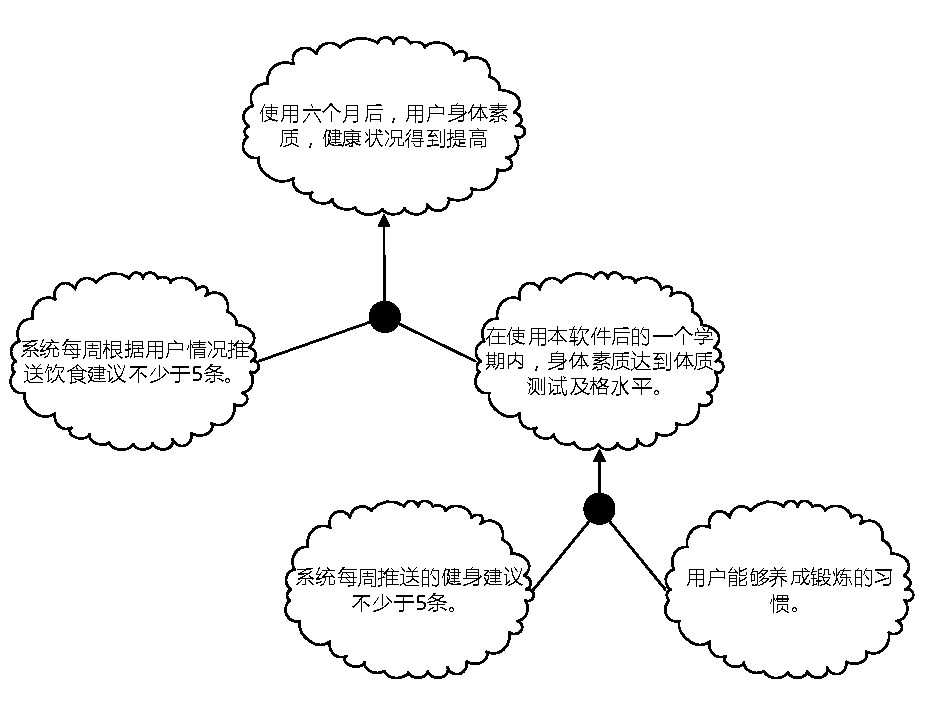
\includegraphics[scale=0.90]{br.pdf}

\section{目标精化}
\subsection{获取对高层次目标的描述}

\subsection{从高层次目标描述中发现AND精化关系}
\subsection{从高层次目标描述中发现OR精化关系}
\subsection{考虑阻碍目标实现的情况}
\subsection{发现目标冲突关系}
\subsection{完善层次结构}

\section{目标实现}
\subsection{将底层目标分配给主体}
\subsection{设计最底层目标的操作(任务)}


\end{document}
